\documentclass[pdftex,12pt,a4paper]{report}
\usepackage[light,math]{iwona}
\usepackage[usenames,dvipsnames]{color}
\usepackage{tikz}
\usepackage{graphicx}
\usepackage{setspace}
\usepackage{natbib}
\newcommand{\HRule}{\rule{\linewidth}{0.5mm}}
\usetikzlibrary{calc,shapes,arrows,automata,trees,shadows,decorations.pathmorphing,positioning, shapes.misc,shapes.arrows,chains,matrix,scopes,decorations.pathmorphing,backgrounds}
\begin{document}
%
\begin{titlepage}
\begin{center}
% Upper part of the page


\textsc{\color{Sepia}{\LARGE EC~320}}\\[1.5cm]
\textsc{\Large Week~One}\\[0.5cm]
\textsc{\Large Question~One}\\[0.5cm]
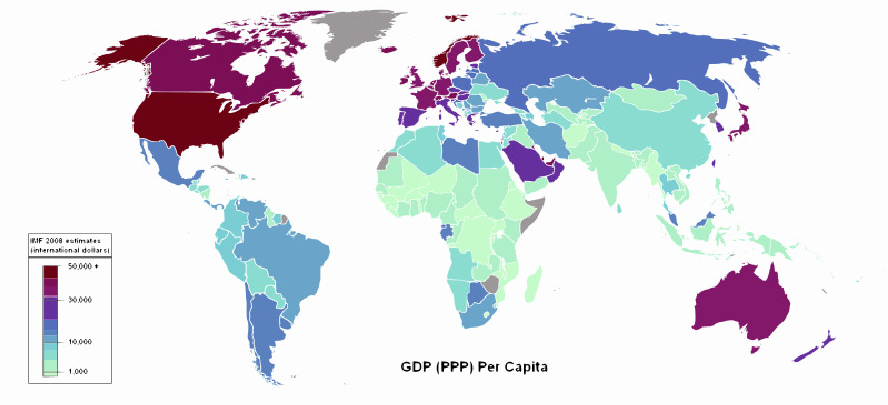
\includegraphics[scale=0.5]{GDP}\\
\cite{wiki:001}
% Title
\HRule \\[0.4cm]
{ \huge \bfseries Principles of Macroeconomics}\\[0.4cm]
\HRule \\[1.5cm]


% Author and supervisor
\begin{minipage}{0.4\textwidth}
\begin{flushleft} \large
\emph{Author:}\\
Jason \textsc{Mansfield}
\end{flushleft}
\end{minipage}
\begin{minipage}{0.4\textwidth}
\begin{flushright} \large
\emph{Instructor:} \\
Dr.~Anthony \textsc{Pizur}
\end{flushright}
\end{minipage}

\vfill

% Bottom of the page
{\large \today}

\end{center}
\end{titlepage}
%
\section{Protectionist}
\begin{doublespace}
I was astonished when reading from the Journal of International Economics~\citep*{blanchard2011escaping} concerning some of the defining factors which purposedly drive voters choices regarding two extreme views of either protectionist  or liberal. The premise is that older workers with skill are more biased to free trade while unskilled older workers are more likely to favor protectionist policies:
\end{doublespace}
\begin{quote}
Adopting the developed country perspective, we show that in an economy with comparative advantage in skill-intensive products, skilled older workers favor free trade, while unskilled, import-competing older workers favor trade barriers.1 The pivotal young generation splits the vote, with lower ability workers supporting protectionism and higher ability workers favoring open markets.
\end{quote}
\begin{doublespace}
Other Journals claim that the great Depression was caused by or deeped the Great Depression of 1929~\citep*{bussière2011protectionist}:
\end{doublespace}
\begin{quote}
The consequences of a rise in protectionism are potentially very substantial. The outburst of protectionism that followed the 1929 market crash is considered to have contributed to the propagation of the crisis and to a marked worsening of the Great Depression (Kindleberger, 1986). Between 1929 and 1933, world trade followed a downward spiral and ultimately contracted by 66\% (Figure 2). The protectionist policies implemented at the time of the Great Depression took a variety of forms. The most cited example of such measures is perhaps the sharp increase in tariffs on US imports introduced by the Smoot-Hawley Act on 17 June 1930, but many other non-tariff measures were introduced, including quotas, “competitive” exchange rate devaluations, export subsidies, and other indirect measures (Eichengreen and Irwin, 2009).
\end{quote}
\subsection{Laissez-faire}
\begin{doublespace}
Economic liberalism promotes laissez-faire which opens the doors to economic freedom. Economic freedom in turn allows us to maintain competitive economic growth as discussed in this article at the Cato Institute~\citep*{lawson2011economic}:
\end{doublespace}
\begin{quotation}
The study also shows that economic freedom is strongly linked with both higher levels of income and faster rates of economic growth. The people living in the top one-fifth of the most free countries enjoy an average income of \$23,450 and a growth rate in the 1990s of 2.56 percent per year; in contrast, the bottom one-fifth in the rankings had an average income of just \$2,556 and a -0.85 percent growth rate in the 1990s.
\end{quotation}
\section{Wages}
\begin{doublespace}
Once again a study by the European University Institute~\citep*{helpman2011trade} shows a large difference in wages between skilled and non-skilled workers:
\end{doublespace}
\begin{quote}
Larger, more-productive firms, screen workers more intensively to exclude those with low-ability. As a result, they have workforces of higher average ability and they pay higher wages. These differences in firm characteristics are systematically related to export participation. Exporters are larger and more productive than non exporters; they screen workers more intensively; and they pay higher wages in comparison to firms with similar productivity that do not export. The resulting framework highlights a new mechanism through which trade affects inequality, based on variation in wages across firms and the participation of only the most-productive firms in exporting.
\end{quote}
\begin{doublespace}
There are of course multiple models out there which conflict or at least do not completely agree with the aforementioned views. The few journals and articles I have read seem to agree life is good for skilled workers and a free flowing economy uninhibited by government is wiser. Its possible life is then better for unskilled workers as someone must pay for unemployment in this capitalist type world? Its hard to define how accurate these studies are simply due to the fact that there is no definition on what skills they are referring to exactly. I suppose that another topic all together?
\end{doublespace}
\clearpage
% bib stuff
    \nocite{*}
    \bibliographystyle{apalike}
    \bibliography{cite}

\end{document}